\subsection{Thermal Radiation and Low-Mass Dileptons}
        \label{Sec:EM}

Electromagnetic (EM) radiation from the fireballs created in heavy-ion collisions
has long been recognized as a valuable probe of hot and dense
matter~\cite{Feinberg:1976ua,Shuryak:1978ij}. Once produced, photons and dileptons
traverse the fireball and reach the detectors without further
re-interaction. Therefore, their measured spectra are direct signals from the hot and dense
phases of the fireball. In particular, thermal radiation from the locally equilibrated
matter contains unique information about the QCD medium.

The physics potential of EM radiation can be gleaned from the expression for its
local emission rate. At a temperature $T$ it is given by
\begin{equation}
R_{\rm EM} = {\rm const} \ f(E;T) \ \rho_{\rm EM}(M,p;T)
\label{eq:rate}
\end{equation}
where $f(E;T)\simeq \exp(-E/T)$ is the thermal distribution function and
$\rho_{\rm EM}(M,p;T)$ the EM spectral function; $M$ is the invariant mass of the
dilepton ($M$=0 for photons), $p$ its 3-momentum and $E=\sqrt{M^2+p^2}$ its energy.
The mass dependence of $\rho_{\rm EM}$ reflects the operational degrees of freedom:
in vacuum, the low-mass region ($M\le 1$~GeV) is saturated by the light vector mesons
$\rho$, $\omega$ and $\phi$, while the intermediate-mass region (1.5~$\le M/\GeV \le$~3)
is characterized by a perturbative quark-anti-quark continuum.

Calculations of thermal dilepton and photon spectra suitable for comparison to
experiment require the emission rate, Eq.~(\ref{eq:rate}), to be integrated over a
realistic space-time evolution of the fireball in heavy-ion collisions, e.g., by
using hydrodynamic models. The following properties of the QCD medium can then be
studied with EM emission spectra in heavy-ion collisions.
\begin{description}
\item[In-Medium Properties of Vector Mesons.]
In the low-mass region, dilepton radiation from the fireball monitors the
medium effects on the vector mesons as the QCD phase transition is approached and
surpassed. In the vacuum, the properties of light hadrons are governed by the
spontaneously broken chiral symmetry induced by the formation of a quark-anti-quark
condensate. The reduction of the condensate in the QCD medium~\cite{Borsanyi:2010bp}
therefore imposes marked changes on the hadron spectrum. Low-mass dileptons are a
unique observable to measure these modifications in the vector meson mass spectrum.
\item[Temperature of the Fireball.]
Dilepton spectra in the intermediate-mass region\linebreak
($1.5 \le M/\GeV \le 3$) provide a
pristine thermometer of the fireball. Since the medium modifications of the continuum
in the EM spectral function, $\rho_{\rm EM}$, are small (suppressed by the ratio
$T^2/M^2$), the spectral slope of the radiation is solely determined by the temperature
in the thermal distribution function, $f(E;T)\simeq{\rm e}^{-E/T}$. For large masses,
its exponential form strongly favors radiation from the hottest phases of the
fireball~\cite{Shuryak:1980tp,Rapp:2004zh}, so that the observed spectra are mostly
emitted from early in the evolution. Since the mass spectra are
Lorentz-{\em invariant}, they are not distorted by a Doppler shift
from the collective expansion of the exploding fireball.
\item[Lifetime of the Fireball.]
The total yields of thermal EM radiation are a measure of the total lifetime of the
emitting fireball (the expanding 3-volume is constrained by final-state hadron yields).
The optimal mass window for this measurement appears to be
$M\simeq$\,0.3-0.7\,GeV~\cite{Rapp:2014hha}, where the radiation yields turn out to
be proportional to the fireball lifetime within about 10\%,
over a large range of heavy-ion collision energies~\cite{Rapp:2014hha}.
\item[Collective Properties of the Emission Source.]
In contrast to the invariant-mass spectra, the transverse-momentum spectra of dileptons
and photons are subject to a Doppler shift: the expansion velocity of the medium
imparts additional energy on the photons and dileptons which makes their spectra appear
``hotter". The slope of the transverse-momentum spectra is therefore determined by both
the temperature and collective-flow properties of the emitting source.
Another powerful observable is the elliptic flow of the EM radiation. Since the elliptic
flow of the bulk medium takes several fm/c to build up, the elliptic flow of the EM
radiation further constrains the origin of its emission.
\end{description}

The physics potential of accurate dilepton data has been demonstrated by the NA60
collaboration at the CERN SPS in collisions of medium-sized nuclei (Indium with A=114)
at an energy of
$\sqrt{s_{NN}}$=17.3\,GeV~\cite{Arnaldi:2008fw,Arnaldi:2008er,Specht:2010xu}. The
low-mass spectra confirmed the gradual melting of the $\rho$-meson resonance into a
structureless quark-anti-quark continuum, while the total yields translate into an
average fireball lifetime of $7\pm1$\,fm/c. The inverse slope of the radiation at
intermediate masses gives an average temperature of $205\pm12$\,MeV, signaling QGP
radiation. The radial-flow pattern in the transverse-momentum spectra confirms
predominantly hadronic and QGP sources at low and intermediate masses, respectively.
Broad dilepton measurements at different energies with heavy projectiles are needed
to exploit this potential for systematic studies across the QCD phase diagram.

\begin{figure}[tbh]
\centerline{
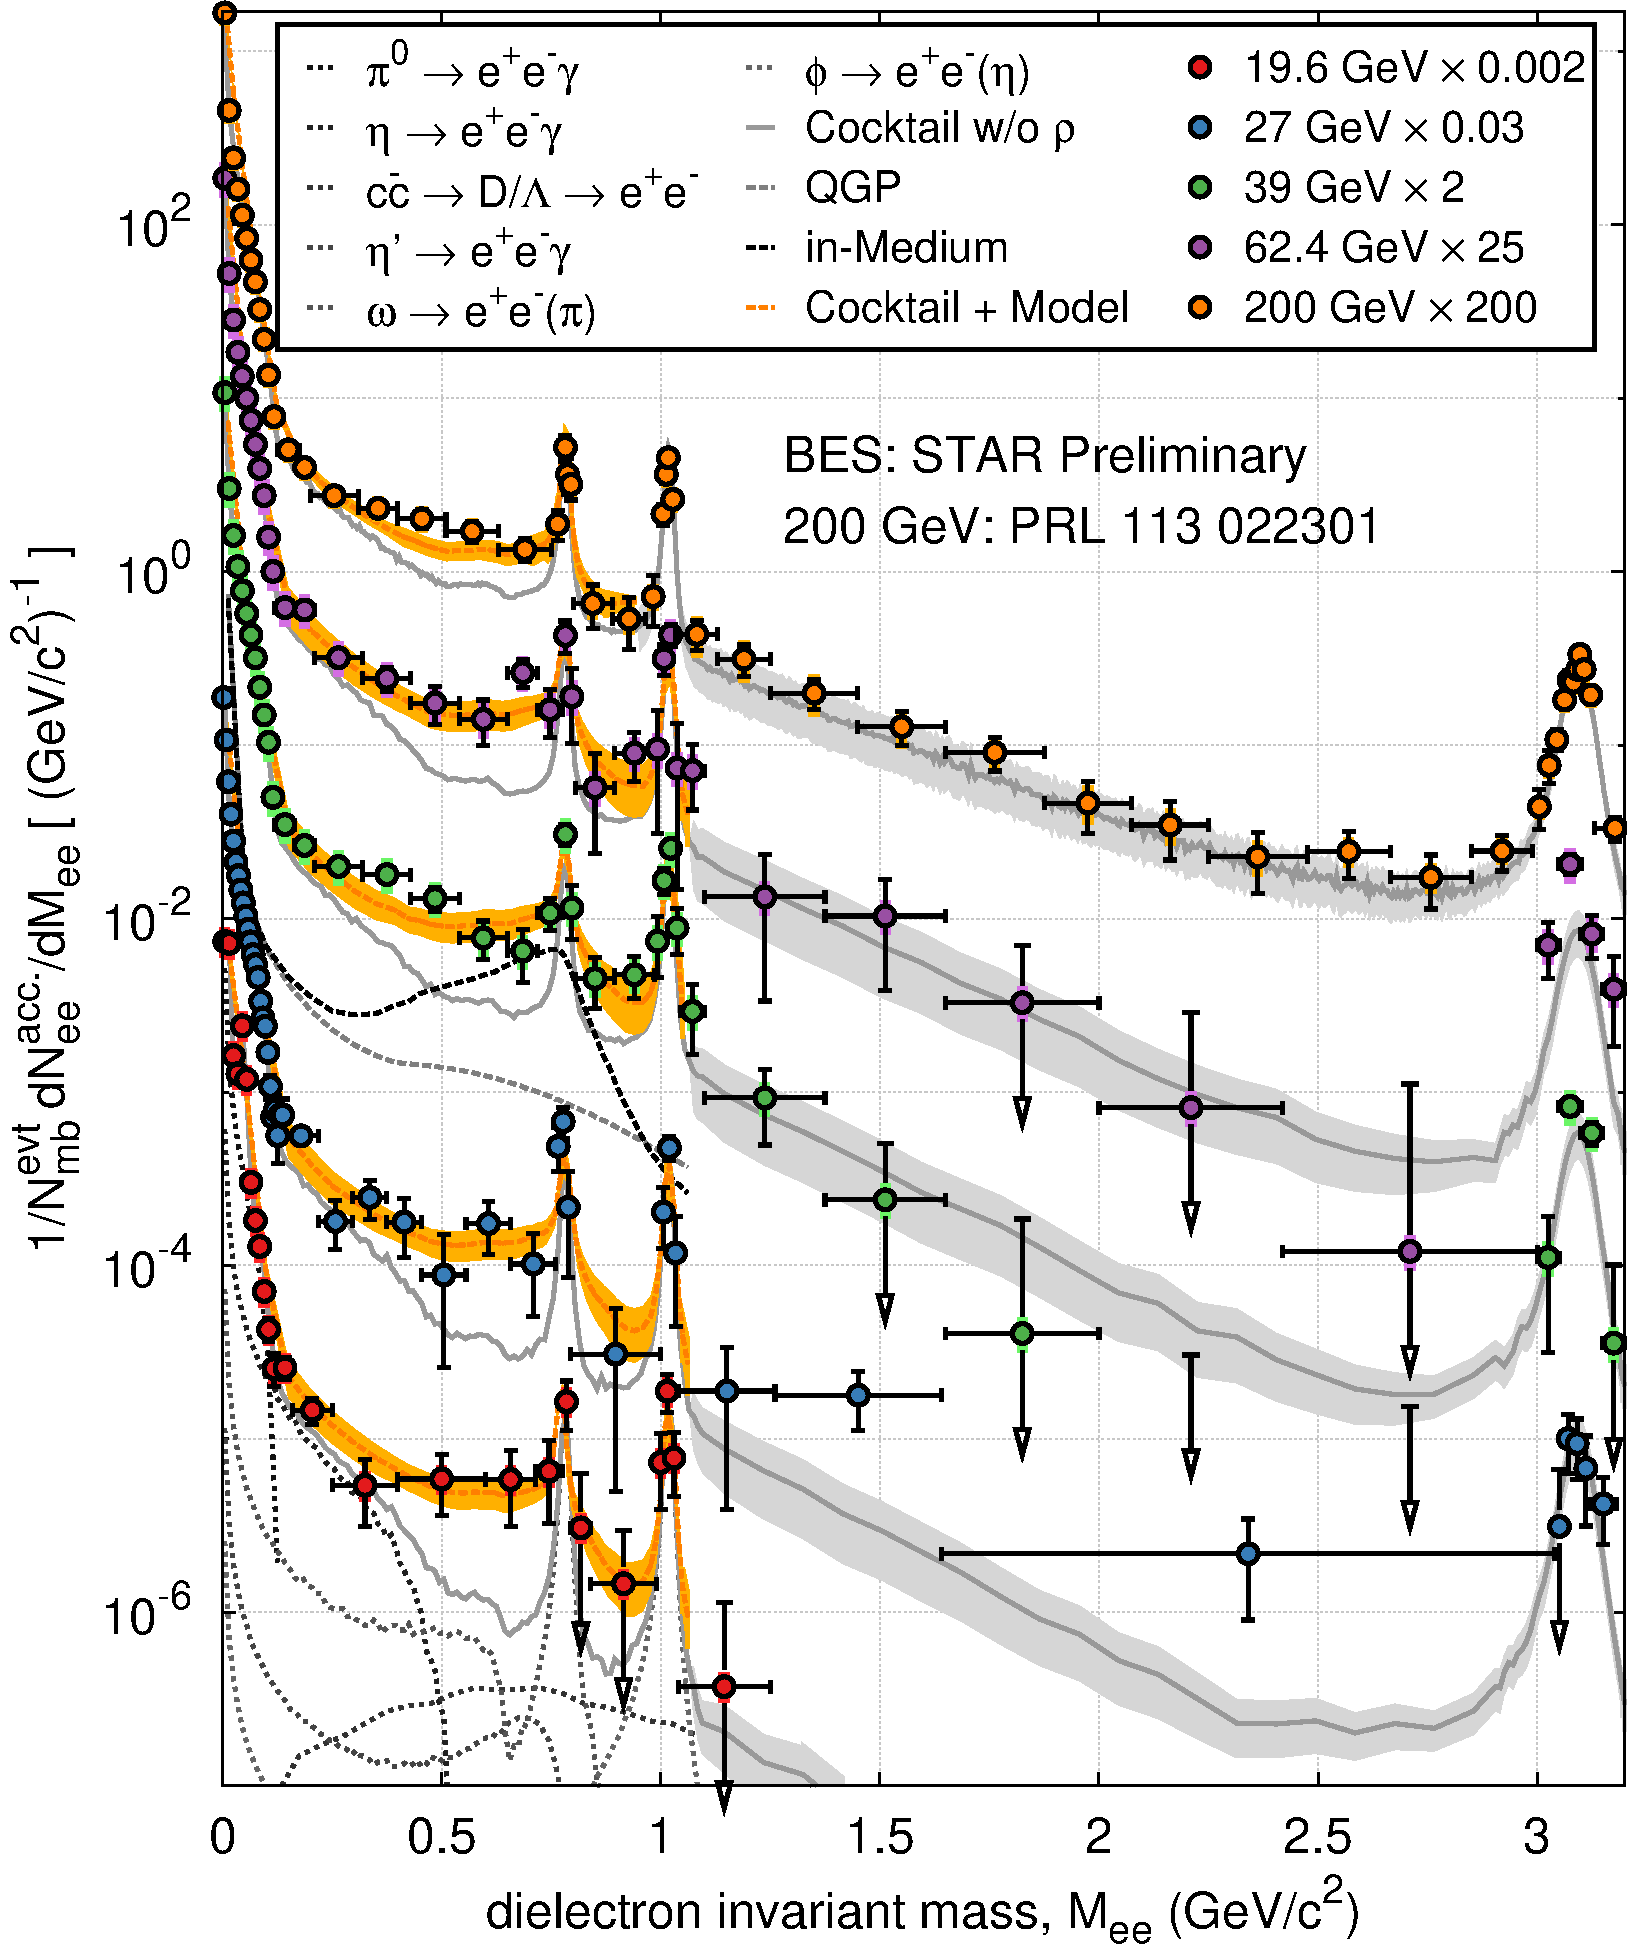
\includegraphics[width=0.45\textwidth]{fig/dNeedM-star}
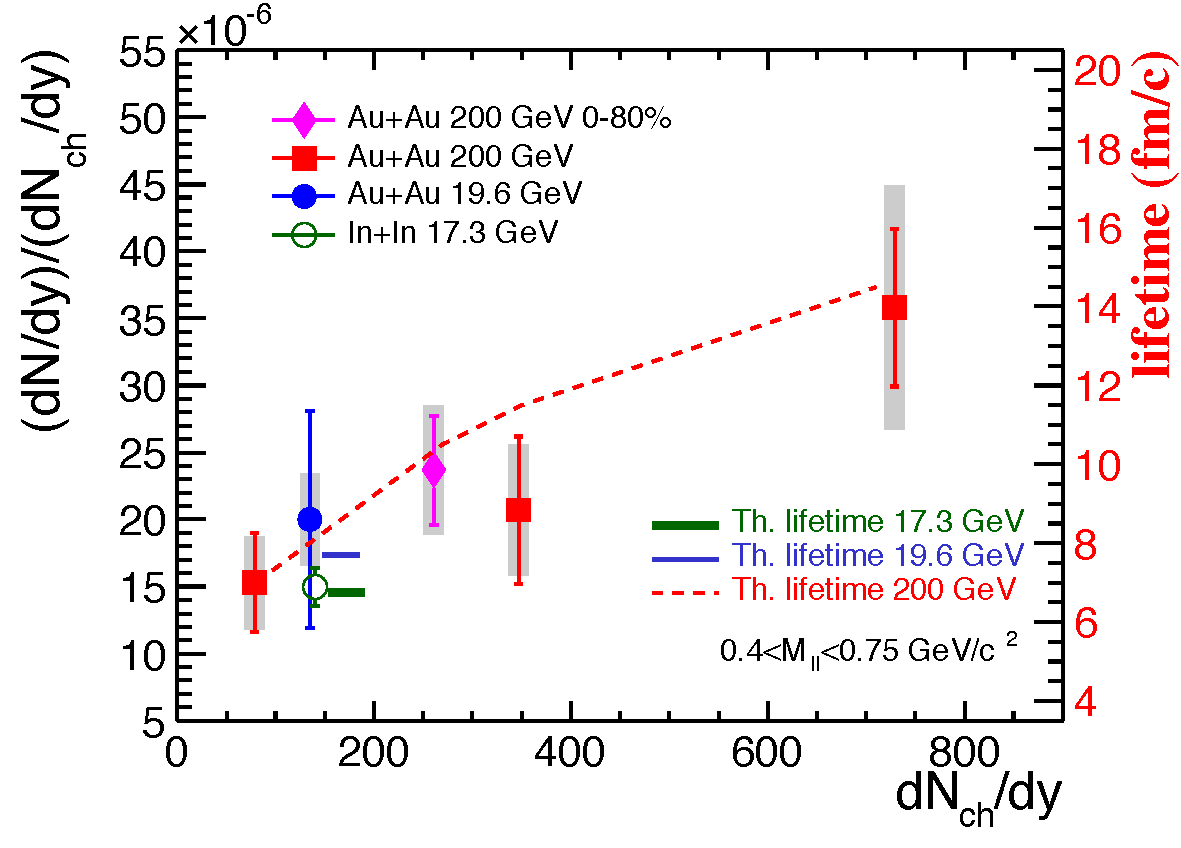
\includegraphics[width=0.55\textwidth]{fig/excessLMRTheoryComp_tau1}
}
\caption[STAR Beam Energy Scan results on di-electron yields]{Di-electron invariant-mass spectra as measured by
STAR~\cite{Adamczyk:2013caa,Huck:2014mfa} in \AuAu\ collisions in the first beam
energy scan at RHIC. The left panel shows the invariant-mass spectra for increasing
collision energies (bottom to top); the orange bands represent the sum of theoretically
predicted thermal radiation~\cite{Rapp:2013nxa} from QGP and hadronic matter
and final-state hadron decays (including their uncertainty). At intermediate masses
($M>1$\,GeV) the spectra are dominated by correlated heavy-flavor decays and are not yet
sensitive to thermal radiation. 
%The right panel shows the dielectron
%transverse pair momentum spectra in the low mass range, $0.4<M/\GeV<0.76)$, again compared
%to the sum (solid line) of thermal radiation and final-state hadron decays.
The right panel shows integrated yields of the normalized dilepton excesses 
for $0.4<M_{ll}<0.75$ GeV/$c^{2}$ as a function of $dN_{\rm ch}/dy$~\cite{Adamczyk:2015bha,Specht:2010xu}. 
The theoretical lifetimes inferred from a model calculation~\cite{Rapp:2014hha} are also shown
}
\label{fig:star-ee}
\end{figure}
A first step in this direction has recently been made by
STAR~\cite{Adamczyk:2013caa,Huck:2014mfa,Adamczyk:2015bha} in the BES program at RHIC. In \AuAu\
collisions covering energies from SPS to top RHIC ($\sqrt{s_{NN}}$=19.6, 27, 39, 62, 200\,GeV),
a sustained low-mass excess radiation was found, cf.~Figure~\ref{fig:star-ee}.
Both mass and transverse-momentum spectra are well described by thermal radiation from
hadronic matter and QGP~\cite{Rapp:2013nxa} (added to contributions from final-state
hadron decays). The data corroborate the melting of the $\rho$  as a robust mechanism of the low-mass
excess in the hadron-to-quark transition at small and moderate baryon chemical potential.
Improved measurements of the low-mass spectral shape at small chemical
potential~\cite{Adamczyk:2013caa} will be critical to discriminate theoretical
models~\cite{Rapp:2000pe,Dusling:2007su,Linnyk:2011vx,Xu:2011tz,Vujanovic:2013jpa}.
This is expected from upcoming high-luminosity \AuAu\ running at 200\,GeV. Lifetime
``measurements" via the integrated low-mass excess require less precision. 
Comparison of 
the BES-I data at $\sqrt{s_{NN}} = $ 19.6 and 200 GeV to theoretical models indicate
that the normalized excess dilepton yields in the low mass region are proportional to the calculated lifetimes of the medium, 
as shown in the right panel of Figure~\ref{fig:star-ee}.
These measurements can be performed with much improved precision in the upcoming BES-II campaign, 
providing a tool to
detect lifetime ``anomalies" possibly induced in the vicinity of a critical
point~\cite{Rapp:2014hha}.

Theoretical progress has been made in elaborating the connection of the dilepton data
to chiral symmetry restoration~\cite{Hohler:2013eba}. The broadening $\rho$-meson
spectral function used to describe the dilepton spectra has been tested  with Weinberg
and QCD sum rules which relate vector and axial-vector spectral functions to quark and
gluon condensates. With temperature-dependent condensates taken from
lattice QCD~\cite{Borsanyi:2010bp}, solutions for the axial-vector spectral function
were found which accurately satisfy the in-medium sum rules. Thus the melting of the
$\rho$-meson resonance is compatible with (the approach to) chiral symmetry restoration.
Further progress has been made in evaluating the in-medium vector correlation function,
and the associated thermal dilepton rates, in thermal lattice
QCD~\cite{Ding:2010ga,Brandt:2012jc}. The computed correlation functions in the QGP
encode a low-mass enhancement which is quite compatible with the spectral functions
that figure into the explanation of the observed dilepton spectra~\cite{Rapp:2011is}.

\begin{figure}[tbh]
\centerline{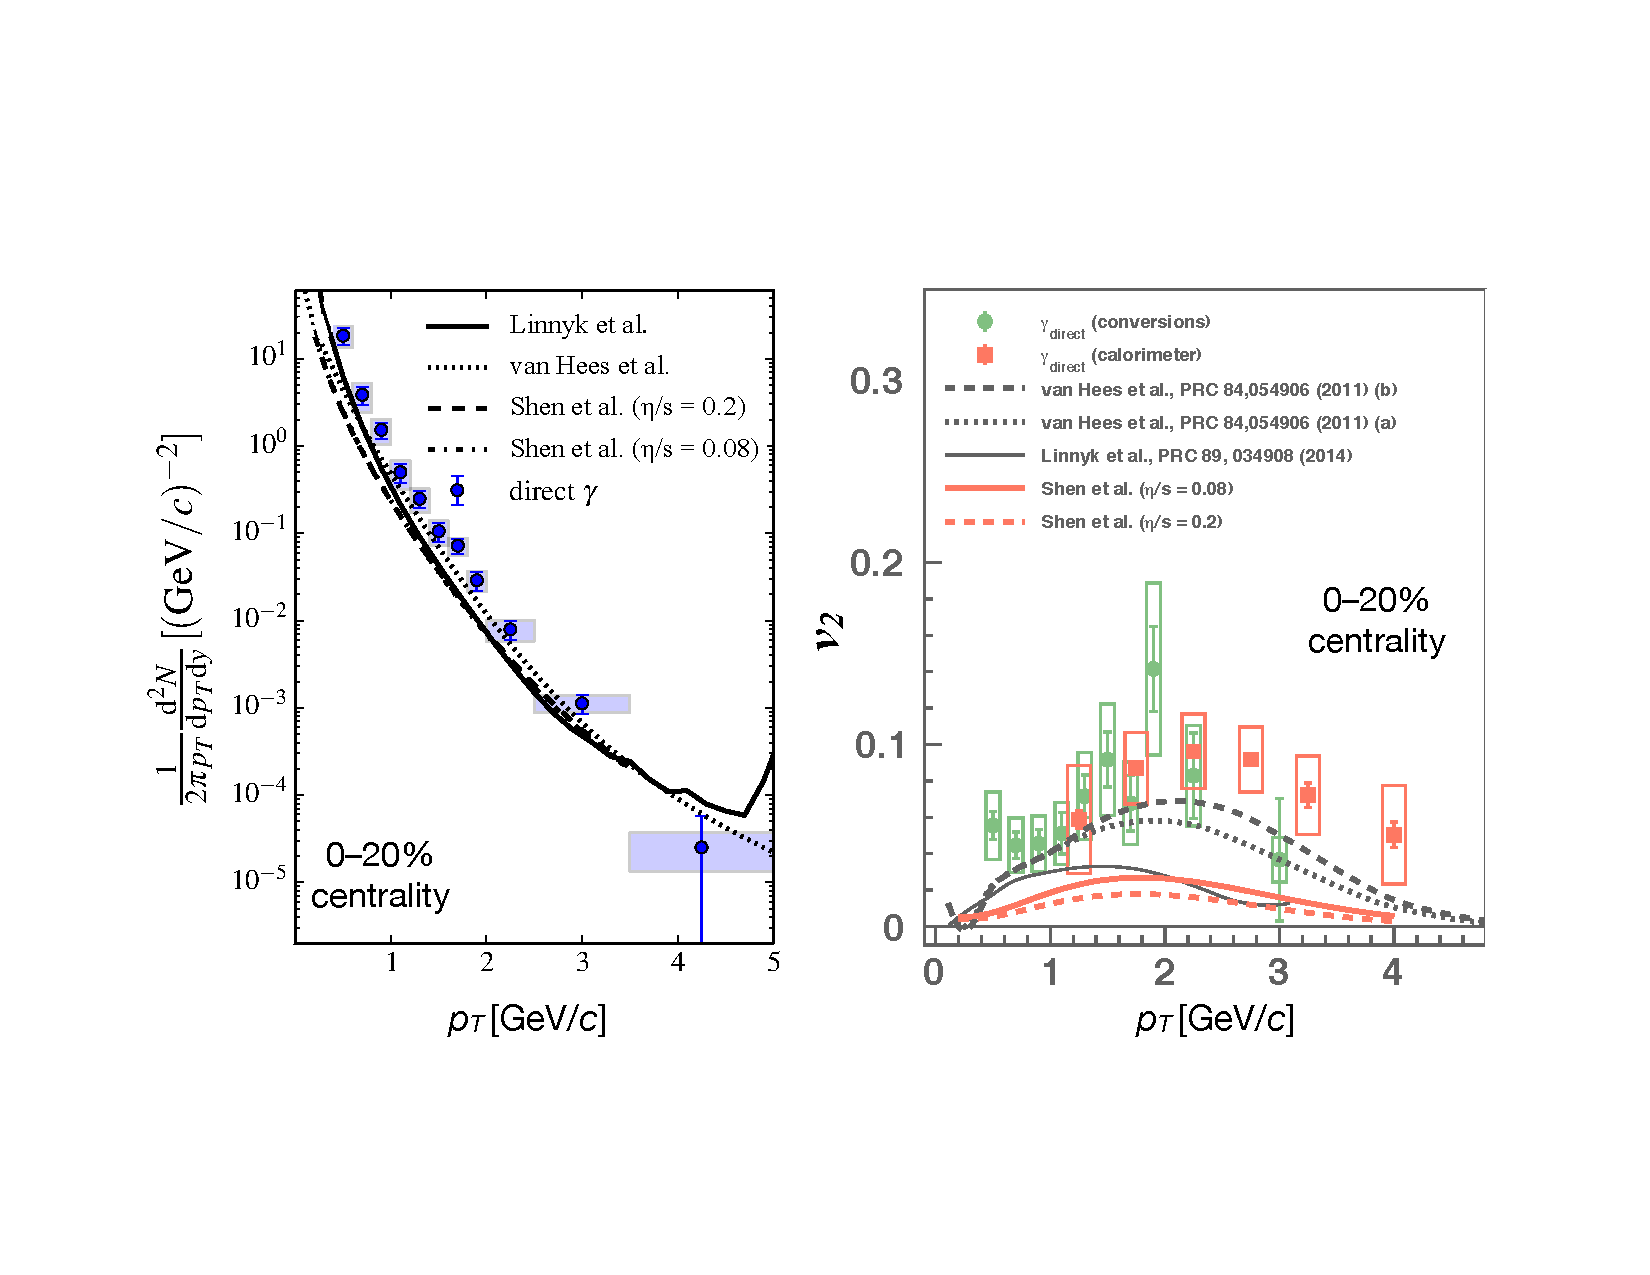
\includegraphics[width=1.0\textwidth]{fig/gam-spec-v2-phenix} }
\caption[PHENIX results on direct photon spectra and flow compared to theory]{Direct photon spectra (left panel) and their elliptic flow (right panel) in 0-20\%
\AuAu\ collisions at 200\,GeV energy. PHENIX data~\cite{Adare:2011zr,Adare:2014fwh,Bannier:2014bja}
are compared to theoretical model calculations~\cite{vanHees:2011vb,Shen:2013cca,Linnyk:2013wma}.
}
\label{fig:phenix-gam}
\end{figure}
An excess signal of low-momentum direct photons, beyond expectations from binary
nucleon-nucleon collisions and final-state hadron decays, has been measured by
PHENIX~\cite{Adare:2008ab} in 200\,GeV \AuAu\ collisions. The transverse momentum spectra of 
the excess photons are of exponential shape with an inverse slope parameter 
$T_{\rm slope}\simeq 240\pm 30$\,MeV~\cite{Adare:2008ab,Adare:2014fwh}.
As noted above, Doppler shifts due to the collective medium expansion need to be accounted for
in extracting the temperature. Theoretical models suggest that the emission mainly originates
from the later QGP and hadronic stages of the fireball, from a rather broad window of
temperatures around $T_{\rm pc}\simeq170$\,MeV, with an average medium expansion velocity of
$\sim$0.3-0.5$c$~\cite{vanHees:2011vb,Shen:2013cca}. The experimental yields tend to be
underestimated by currently available calculations for thermal radiation, as shown in the left
panel of Figure~\ref{fig:phenix-gam}. Similar measurements are also becoming available
from STAR~\cite{Yang:2014mla}.

The direct photon excess carries a surprisingly large elliptic flow
($v_2$)~\cite{Adare:2011zr,Bannier:2014bja} as seen in the right panel of Figure~\ref{fig:phenix-gam}.
In fact, the magnitude of the flow is comparable to that of pions, which are emitted
when the fireball decouples. This is incompatible with
a large contribution to the direct photon excess from early QGP
radiation~\cite{Chatterjee:2005de,Liu:2009kta,Holopainen:2011pd,vanHees:2011vb,Dion:2011pp,Shen:2013cca,Linnyk:2013wma},
and again points to a later emission of the excess photons. The elliptic flow strength $v_2$ also is underestimated
by current theoretical calculations, but more precise data are needed to quantify the discrepancies.

The PHENIX data have triggered substantial theoretical activity. To obtain sufficiently large yields 
{\em and} a large $v_2$ from a thermal photon source the bulk medium would need to develop its final $v_2$ rather 
rapidly, probably before reaching the phase transition regime~\cite{vanHees:2011vb}. This could be driven, 
e.g., by a pre-equilibrium radial flow from a glasma evolution~\cite{Dusling:2010rm,Chen:2013ksa}.
Such favorable collective properties would also need to be accompanied by large photon rates in the phase transition
regime~\cite{vanHees:2011vb,Shen:2013vja,vanHees:2014ida} and in the hadronic
phase~\cite{Turbide:2003si}. An initially gluon-rich plasma~\cite{McLerran:2014hza}, or 
nonperturbative effects in a QGP~\cite{Gale:2014dfa}, could aid in suppressing
early electromagnetic emission when the bulk $v_2$ is still small
and thereby avoid diluting the observed strong $v_2$ pattern with the azimuthally symmetric
distribution expected for photons emitted early in the collision.

Preliminary measurements of the direct-photon triangular flow ($v_3$)~\cite{Bannier:2014bja}
support a thermal emission source~\cite{Shen:2013cca} and disfavor more exotic sources, e.g.,
from strong but short-lived primordial magnetic fields~\cite{Basar:2012bp,Bzdak:2012fr}.
The centrality dependence of the excess signal~\cite{Adare:2014fwh} is consistent
with expectations from thermal radiation, but is also compatible with scaling arguments based on
initial-state saturation effects~\cite{McLerran:2014oea}. Improved measurements of the
photon spectra and their collective properties will be critical in resolving these issues, as will 
be extending these measurements to other colliding systems. 

Closely related but independent observables are the transverse-momentum spectra and $v_2$ of
low-mass dileptons.
A first measurement of
the $v_2$ has been achieved~\cite{Adamczyk:2014lpa} but does not yet provide tangible
discrimination power. 
Again, improved and extended experimental measurements are required, as well
as additional calculations. Since photons and dileptons are intimately related in theoretical
calculations, a complete understanding of EM data and its implications for the thermal 
history of the medium will need to account for both observables
simultaneously.
